\documentclass[9pt]{beamer}
\usetheme{Boadilla}

\makeatother
\setbeamertemplate{footline}
{
	\leavevmode%
	\hbox{%
		\begin{beamercolorbox}[wd=.4\paperwidth,ht=2.25ex,dp=1ex,center]{author in head/foot}%
			\usebeamerfont{author in head/foot}\insertshortauthor
		\end{beamercolorbox}%
		\begin{beamercolorbox}[wd=.6\paperwidth,ht=2.25ex,dp=1ex,center]{title in head/foot}%
			\usebeamerfont{title in head/foot}\insertshorttitle\hspace*{3em}
			\insertframenumber{} / \inserttotalframenumber\hspace*{1ex}
	\end{beamercolorbox}}%
	\vskip0pt%
}
\makeatletter
\setbeamertemplate{navigation symbols}{}

\usepackage{tikz}
\usetikzlibrary{positioning}

\usepackage{lipsum}
\usepackage{appendixnumberbeamer}

\usepackage[authoryear]{natbib}
\usepackage[latin1]{inputenc}
\usepackage[T1]{fontenc}
\usepackage{caption}
\usepackage{amsmath, amssymb}
\usepackage{epstopdf}
\usepackage{graphicx}
\usepackage{lmodern}
\usepackage{xcolor}
\usepackage{xpatch}
\usepackage{multirow}

\usepackage{amsmath,theorem,amssymb,graphicx, pgfplots, tabularx, placeins}
\usepackage{dsfont}
\usepackage{caption}
%\usepackage{subcaption}
\setbeamertemplate{caption}{\raggedright\insertcaption\par}
%\setbeamertemplate{footline}[frame number]
\usepackage{csquotes}
\usepackage{bm}
\bibliographystyle{econometrica}
\usepackage[normalem]{ulem}

\usepackage{setspace}


\definecolor{gray(x11gray)}{rgb}{0.75, 0.75, 0.75}


\newcommand{\bit}{\begin{itemize}}
	\newcommand{\eit}{\end{itemize}}
\newcommand{\ben}{\begin{enumerate}}
	\newcommand{\een}{\end{enumerate}}


\newcommand{\bc}{\color{blue}}
\newcommand{\rc}{\color{red}}

\newcommand{\lb}{\label}
\newcommand{\re}{\eqref}

\title[Incomplete markets models: basics]{Macroeconomics II, Lecture XI:\\
	 Incomplete markets models: basics}
\author{Erik {\"O}berg}
\date{}

\begin{document}

\maketitle


\begin{frame}{Introduction}

\bit
\setlength\itemsep{1.5em}

\item Traditional macroeconomic models assumes a representative agent: \bf no room for studying the interaction between macroeconomic dynamics and inequality \normalfont

\item Inequality/economic heterogeneity is, however, a very salient feature of the macroeconomic environments we seek to understand

\item In the last part of this course, we will study macroeconomic models with {\bc heterogeneous households}
\bit
	\item Alternatively, macroeconomic models with {\bc incomplete asset markets}
\eit

\item We use these models to investigate:
\ben
\setlength\itemsep{1 em}
\item distributional implications of macroeconomic events
\bit
\item Does technical change increase income inequality?
\item Does wealth inequality widen when credit become cheaper?
\eit

\item how household heterogeneity matter for macroeconomic transmission
\bit
\item Does wider wealth inequality imply more business cycle volatility?
\item Does the existence of more high-debt household imply that monetary policy is more potent?
\eit
\een

\eit

\end{frame}



\begin{frame}{US cross-sectional wage inequality}

\begin{figure}
	\centering
	\includegraphics[scale=0.45]{figures/hpv_2010_wageinequality.pdf}
	\caption*{\footnotesize From Heathcote-Perri-Violante (RED 2010) using CPS data}
\end{figure}

\end{frame}

\begin{frame}{US top income share}

\begin{figure}
	\centering
	\includegraphics[scale=0.4, trim = 0cm 3cm 0cm 0cm, clip]{figures/piketty_inc_ineq.pdf}
	\caption*{\footnotesize From Piketty (Book 2014) using US register data}
\end{figure}


\end{frame}

\begin{frame}{US income inequality over the life-cycle}

\begin{figure}
	\centering
	\includegraphics{figures/guvenen_2016_lifecycle.pdf}
	\caption*{\footnotesize From Guvenen-Karahan-Ozkan-Song (Ecmtra 2021) using US register data}
\end{figure}


\end{frame}

\begin{frame}{Income inequality widens in recessions}

\begin{figure}
	\centering
	\includegraphics[scale=0.5]{figures/guvenen_2014_recession.pdf}
	\caption*{\footnotesize From Guvenen-Ozkan-Song (JPE 2014) using US register data}
\end{figure}


\end{frame}



\begin{frame}{US income and wealth inequality}

\begin{figure}
	\centering
	\includegraphics[scale=0.8, trim = 0cm 0cm 0cm 0cm, clip]{figures/kuhn2020_fig4.pdf}
	\caption*{\footnotesize From Kuhn-Schularick-Steins (JPE 2020) using SCF+ data}
\end{figure}

\end{frame}



\begin{frame}{Course part III outline}

\bit
\setlength\itemsep{2em}

\item Lecture 11: Incomplete markets models: basics

\item Lecture 12: Buffer-stock savings: model meet data

\item Lecture 13: Incomplete markets in general equilibrium


\eit

\end{frame}



\begin{frame}{Today's agenda}

\ben
\setlength\itemsep{2em}

\item Aggregation under different market structures
	\bit
	\setlength\itemsep{0.5em}
		\item Autarky
		\item Complete markets
		\item Incomplete markets
	\eit

\item Consumption-savings dynamics with incomplete markets
\bit
\setlength\itemsep{0.5em}
	\item The household problem: setup and characterization 
	\item Precautionary savings
\eit

\een

\end{frame}



\begin{frame}

\begin{center}
	\huge Aggregation and market structure \normalfont
\end{center}

\end{frame}


\begin{frame}{A classification of models}

\bit
\setlength\itemsep{1.5em}

\item The interaction between aggregate and distributional dynamics depends on the underlying {\bc market structure}

\item {\bc Market structure} refers to which assets are available to the household --- determines how the household can allocate its resources between different states.

\item The household budget constraint in three benchmark structures:
\ben
\setlength\itemsep{2em}

\item \bf Autarky:
\begin{eqnarray}
C_{it}(s^t) \leq Y_{it}(s^t) \hspace{3mm} \forall t,s^t \nonumber 
\end{eqnarray}

\item Complete markets:
\begin{eqnarray}
C_{it}(s^t) + \sum_{s_{t+1}|s^t} Q_t(s^t, s_{t+1}) A_{it+1}(s^t, s_{t+1})  \leq Y_{it}(s^t) + A_{it}(s^t, s_t) \hspace{3mm} \forall t, s^{t}  \nonumber 
\end{eqnarray}

\item (Standard) Incomplete markets: \normalfont
\begin{eqnarray}
C_{it}(s^t) + Q_t(s^t) A_{it+1}(s^t)\leq y_{it}(s^t) + A_{it}(s^{t-1}) \hspace{3mm} \forall t,s^t \nonumber 
\end{eqnarray}
\een

\item Now: quick bird's eye's review of these benchmarks 

\eit

\end{frame}


\begin{frame}{Environment}

\bit
\setlength\itemsep{1.5em}

\item Time is discrete and indexed by $t$

\item The economy has N households indexed by $i$

\item All households lives for $T$ periods; $T = \infty$ is possible

\item One non-storable consumption good

\item In each period, an aggregate event $s_t \in S$ is realized

\item At time $t=0$, each particular event history at time $t$, $s^t = \{s_0, s_1, ..., s_t\} \in S^t$, is realized with probability $\pi(s^t)$

\item Given event history $s^t$ at time $t$, each event at time $t+1$, $s_{t+1} \in S$, is realized with probability $\pi(s_{t+1}|s^t)$

\item For each event history $s^t$, each household $i$ recieves endowment $Y^i_t(s^t)$
\eit

\end{frame}



\begin{frame}{Example event history}

\bit
\item Assume $s_t \in S=\{0,1\}$
\item In period 3, there exists 8 possible ``event histories'' or ``states of the world'':
\eit

\begin{figure}
\begin{center}
	\small
	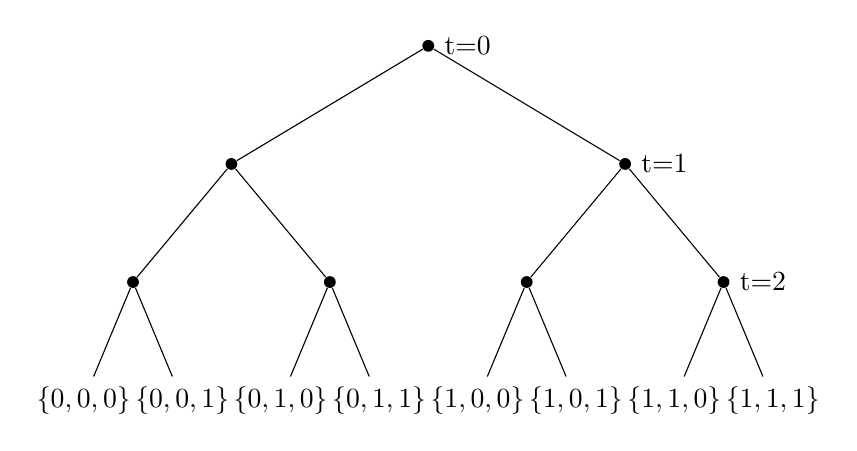
\begin{tikzpicture}[thin,
	level 1/.style={sibling distance=50mm},
	level 2/.style={sibling distance=25mm},
	level 3/.style={sibling distance=12.5mm},
	every circle node/.style={minimum size=1.5mm,inner sep=0mm}]
	
	\node[circle,fill,label=right:$\text{t=}0$] (root) {}
	child { node [circle,fill] {}
		child { node [circle,fill] {}
			child { 
				node {$\{0,0,0\}$}
				edge from parent}
			child { 
				node {$\{0,0,1\}$}
				edge from parent}
			edge from parent}
		child { node [circle,fill] {}
			child { 
				node {$\{0,1,0\}$}
				edge from parent}
			child { 
				node {$\{0,1,1\}$}
				edge from parent}
			edge from parent}
		edge from parent}
	child { node [circle,fill,label=right:$\text{t=}1$] {}
		child { node [circle,fill] {}
			child { 
				node {$\{1,0,0\}$}
				edge from parent}
			child { 
				node {$\{1,0,1\}$}
				edge from parent}
			edge from parent}
		child { node [circle,fill,label=right:$\text{t=}2$] {}
			child { 
				node {$\{1,1,0\}$}
				edge from parent}
			child { 
				node {$\{1,1,1\}$}
				edge from parent}
			edge from parent}
		edge from parent};
	\end{tikzpicture}
\end{center}
\end{figure}

\bit
\item Note 1: Here, individual endowment depends on entire event history, $Y^i_t = Y^i_t(s^t)$ 
\item Note 2: Even if income only depend on the realized shock today, $Y^i_t = Y^i_t(s_t)$, consumption and savings choices in period t depend on the entire event history $s^t$
\eit

\end{frame}



\begin{frame}{Preferences and beliefs}

\bit
\setlength\itemsep{2em}

\item All households have identical preferences: time-separable, common discount factor $\beta$

\item Rational expectations: subjective beliefs about event probabilities coincide with actual probabilities

\item Household objective
\begin{eqnarray} 
U_{i} &=& E_{0} \sum_{t=0}^{T} \beta^t U(C_{it}(s^t)) \nonumber \\
&=& \sum_{t=0}^{T} \sum_{s^t \in S^t} \beta^t \pi (s^t) U(C_{it}(s^t)) \nonumber
\end{eqnarray}

\item $U$ has the usual regularity conditions: twice differentiable, strictly increasing, strictly concave and satisfies the Inada conditions

\eit

\end{frame}

\begin{frame}{Allocations}

\bit
\setlength\itemsep{2em}

\item A consumption allocation is a collection $\{C_{it}(s^t)\}_{i=0}^N$

\item A consumption allocation is feasible if
\begin{eqnarray}
C_{it}(s^t) &\geq& 0 \hspace{3mm} \forall i,t,s^t \nonumber \\
C_t(s^t)  &\leq& Y_t(s^t) \hspace{3mm}  \forall t,s^t \nonumber
\end{eqnarray}
where
\begin{eqnarray}
C_t(s^t) \equiv \sum_{i=1}^{N} C_{it}(s^t), \hspace{2mm} Y_t(s^t) \equiv \sum_{i=1}^{N} Y_{it}(s^t) \hspace{3mm} \nonumber
\end{eqnarray}

\item A feasible consumption allocation $\{C_{it}(s^t)\}_{i=0}^N$ is Pareto efficient if there is no other feasible consumption allocation $\{\hat C_{it}(s^t)\}_{i=0}^N$ such that
\begin{eqnarray}
U(\hat C_{it}(s^t)) &\geq& U(C_{it}(s^t)) \hspace{3mm} \text{for all } i\nonumber \\
U(\hat C_{it}(s^t)) &>& U(C_{it}(s^t)) \hspace{3mm} \text{for some } i\nonumber
\end{eqnarray}

\eit

\end{frame}


\begin{frame}{Autarky}

\begin{figure}
	\begin{center}
		\small
		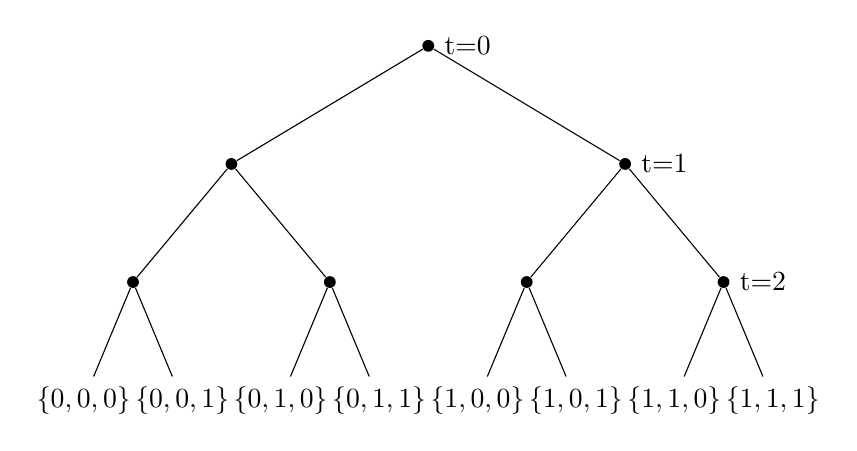
\begin{tikzpicture}[thin,
		level 1/.style={sibling distance=50mm},
		level 2/.style={sibling distance=25mm},
		level 3/.style={sibling distance=12.5mm},
		every circle node/.style={minimum size=1.5mm,inner sep=0mm}]
		
		\node[circle,fill,label=right:$\text{t=}0$] (root) {}
		child { node [circle,fill] {}
			child { node [circle,fill] {}
				child { 
					node {$\{0,0,0\}$}
					edge from parent}
				child { 
					node {$\{0,0,1\}$}
					edge from parent}
				edge from parent}
			child { node [circle,fill] {}
				child { 
					node {$\{0,1,0\}$}
					edge from parent}
				child { 
					node {$\{0,1,1\}$}
					edge from parent}
				edge from parent}
			edge from parent}
		child { node [circle,fill,label=right:$\text{t=}1$] {}
			child { node [circle,fill] {}
				child { 
					node {$\{1,0,0\}$}
					edge from parent}
				child { 
					node {$\{1,0,1\}$}
					edge from parent}
				edge from parent}
			child { node [circle,fill,label=right:$\text{t=}2$] {}
				child { 
					node {$\{1,1,0\}$}
					edge from parent}
				child { 
					node {$\{1,1,1\}$}
					edge from parent}
				edge from parent}
			edge from parent};
		\end{tikzpicture}
	\end{center}
\end{figure}

\bit
\item Autarky: nothing can be traded at any node
\eit

\end{frame}




\begin{frame}{Autarky}

\bit
\setlength\itemsep{1.5em}

\item Household problem:
\begin{eqnarray}
\max_{c(s^t)} && \sum_{t=0}^{T} \sum_{s^t \in S^t} \beta^t \pi (s^t) U(C_{it}(s^t)) \nonumber \\
\text{s.t.} && c_{it}(s^t) \leq y_{it}(s^t) \hspace{3mm} \forall t,s^t \nonumber
\end{eqnarray}

\item Solution to household problem is trivial: $c_{it}(s^t) = y_{it}(s^t) $

\item Distributional dynamics follows mechanically: individual consumption tracks individual income

\item Aggregate dynamics follows mechanically: no prices, and 
\begin{eqnarray}
C_{t}(s^t) = Y_{t}(s^t) \hspace{3mm} \forall t,s^t \nonumber
\end{eqnarray}

\eit

\end{frame}


\begin{frame}{Complete markets (with Arrow securities)}

\begin{figure}
	\begin{center}
		\small
		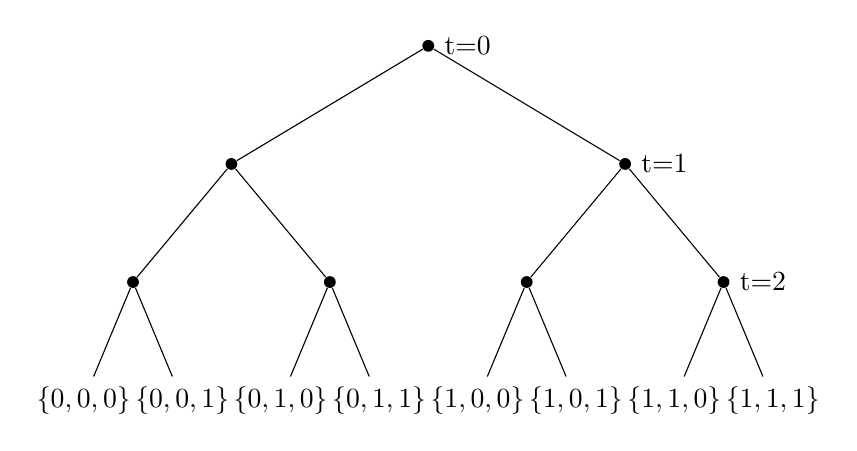
\begin{tikzpicture}[thin,
		level 1/.style={sibling distance=50mm},
		level 2/.style={sibling distance=25mm},
		level 3/.style={sibling distance=12.5mm},
		every circle node/.style={minimum size=1.5mm,inner sep=0mm}]
		
		\node[circle,fill,label=right:$\text{t=}0$] (root) {}
		child { node [circle,fill] {}
			child { node [circle,fill] {}
				child { 
					node {$\{0,0,0\}$}
					edge from parent}
				child { 
					node {$\{0,0,1\}$}
					edge from parent}
				edge from parent}
			child { node [circle,fill] {}
				child { 
					node {$\{0,1,0\}$}
					edge from parent}
				child { 
					node {$\{0,1,1\}$}
					edge from parent}
				edge from parent}
			edge from parent}
		child { node [circle,fill,label=right:$\text{t=}1$] {}
			child { node [circle,fill] {}
				child { 
					node {$\{1,0,0\}$}
					edge from parent}
				child { 
					node {$\{1,0,1\}$}
					edge from parent}
				edge from parent}
			child { node [circle,fill,label=right:$\text{t=}2$] {}
				child { 
					node {$\{1,1,0\}$}
					edge from parent}
				child { 
					node {$\{1,1,1\}$}
					edge from parent}
				edge from parent}
			edge from parent};
		\end{tikzpicture}
	\end{center}
\end{figure}

\bit
\item At each node $s^t$, two assets can be traded: 
\ben
	\item pays of one consumption good at node $\{s^t,0\}$ and costs $Q_t(s^t,0)$
	\item pays of one consumption good at node $\{s^t,1\}$ and costs $Q_t(s^t,1)$ 
\een
\eit

\end{frame}



\begin{frame}{Complete markets}

\bit
\setlength\itemsep{2em}

\item Household problem:
\begin{eqnarray}
\max_{C_{it}(s^t), \{A_{it+1}(s^t, s_{t+1})\}} && \sum_{t=0}^{T} \sum_{s^t \in S^t} \beta^t \pi (s^t) U(C_{it}(s^t)) \nonumber \\
\text{s.t.} && 	C_{it}(s^t) + \sum_{s_{t+1}|s^t} Q_t(s^t, s_{t+1}) A_{it+1}(s^t, s_{t+1})  \leq Y_{it}(s^t) + A_{it}(s^t, s_t) \hspace{3mm} \forall t, s^{t}\nonumber \\
&& A_{it+1}(s^t, s_{t+1}) \geq - \bar A_i \hspace{3mm} \forall t, s^{t}\nonumber
\end{eqnarray}

\item {\bc First welfare theorem} applies: allocation is Pareto efficient and therefore coincides with that of a Social Planner for some Pareto weights $\{\alpha_i\}_{1}^{N}$


\eit

\end{frame}


\begin{frame}{Complete markets implies full insurance}

\bit
\setlength\itemsep{2em}

\item Equilibrium features {\bc full insurance}: {\rc (Do on whiteboard)}
\begin{eqnarray}
\frac{U_c(C_{it}(s^t))}{U_C(C_{jt}(s^t))} \hspace{3mm} = \frac{\alpha_j}{\alpha_i} \hspace{3mm} \forall s^t \nonumber
\end{eqnarray}


\item Full insurance: if my gain from consuming more in some state is high, yours must be high in that state too

\item With CRRA preferences $U(C_{it}(s^t)) = \frac{(C_{it}(s^t))^{1-\sigma}-1}{1-\sigma}$, full insurance implies that the allocation and prices only depend on aggregate consumption:
\begin{eqnarray}
C_{it}(s^t) &=& \theta_i C_{t}(s^t) \nonumber \\
Q_t(s^t, s_{t+1}) &=& \beta \pi(s_{t+1} | s^t) \frac{U_c(C_{t+1}(s^t))}{U_c(C_{t}(s^t))} \nonumber
\end{eqnarray}
%\bit
%	\item Note: log preferences are a special case of CRRA
%\eit

\eit

\end{frame}


\begin{frame}{Complete markets: implications}

\bit
\setlength\itemsep{2em}

\item Hence, the distribution of consumption is constant over time...

\item ... and aggregate dynamics \bf \emph{as if} \normalfont representative agent who solves
\begin{eqnarray}
\max_{C_{t}(s^t), A_{t+1}(s^t)} && \sum_{t=0}^{T} \sum_{s^t \in S^t} \beta^t \pi (s^t) U(C_{t}(s^t)) \nonumber \\
\text{s.t.} && 	C_{t}(s^t) + \sum_{s_{t+1}|s^t} Q_t(s^t, s_{t+1}) A_{t+1}(s^t, s_{t+1}) \leq Y_{t}(s^t) + A_{t}(s^t, s_{t-1}) \hspace{3mm} \forall t, s^{t}\nonumber \\
&& A_{t+1}(s^t) \geq - \bar A \hspace{3mm} \forall t, s^{t}\nonumber
\end{eqnarray}

\item $\Rightarrow$ If markets are sufficiently complete, rep-agent macro seems legitimate
\bit
\setlength\itemsep{0.5em}
	\item Large literature testing the extent of consumption insurance, see Violante lecture notes and D Kruegers textbook
	
	\item Violante also discusses more general aggregation results
\eit 

\eit


\end{frame}



\begin{frame}{(Standard) Incomplete markets}

\begin{figure}
	\begin{center}
		\small
		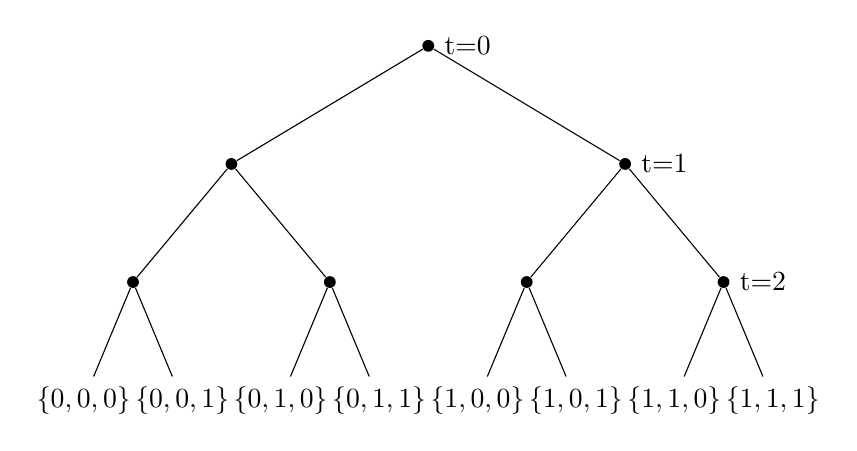
\begin{tikzpicture}[thin,
		level 1/.style={sibling distance=50mm},
		level 2/.style={sibling distance=25mm},
		level 3/.style={sibling distance=12.5mm},
		every circle node/.style={minimum size=1.5mm,inner sep=0mm}]
		
		\node[circle,fill,label=right:$\text{t=}0$] (root) {}
		child { node [circle,fill] {}
			child { node [circle,fill] {}
				child { 
					node {$\{0,0,0\}$}
					edge from parent}
				child { 
					node {$\{0,0,1\}$}
					edge from parent}
				edge from parent}
			child { node [circle,fill] {}
				child { 
					node {$\{0,1,0\}$}
					edge from parent}
				child { 
					node {$\{0,1,1\}$}
					edge from parent}
				edge from parent}
			edge from parent}
		child { node [circle,fill,label=right:$\text{t=}1$] {}
			child { node [circle,fill] {}
				child { 
					node {$\{1,0,0\}$}
					edge from parent}
				child { 
					node {$\{1,0,1\}$}
					edge from parent}
				edge from parent}
			child { node [circle,fill,label=right:$\text{t=}2$] {}
				child { 
					node {$\{1,1,0\}$}
					edge from parent}
				child { 
					node {$\{1,1,1\}$}
					edge from parent}
				edge from parent}
			edge from parent};
		\end{tikzpicture}
	\end{center}
\end{figure}

\bit
\item At each node $s^t$, one asset that pays of one consumption good in period $t+1$ and costs $Q(s^t)$ can be traded
\eit

\end{frame}


\begin{frame}{Incomplete markets}

\bit
\setlength\itemsep{2em}

\item Household problem:
\begin{eqnarray}
\max_{C_{it}(s^t), A_{it+1}(s^t)} && \sum_{t=0}^{T} \sum_{s^t \in S^t} \beta^t \pi (s^t) U(C_{it}(s^t)) \nonumber \\
\text{s.t.} && 	C_{it}(s^t) + Q_t(s^t) A_{it+1}(s^t)  \leq Y_{it}(s^t) + A_{it}(s^{t-1}) \hspace{3mm} \forall t, s^{t}\nonumber \\
&& A_{it+1}(s^t, s_{t+1}) \geq - \bar A_i \hspace{3mm} \forall t, s^{t}\nonumber
\end{eqnarray}

\item Due to lack of insurance, ex-ante homogeneous households will be \bf ex-post heterogeneous \normalfont in terms of $\{C,A,Y\}$

\item Due to lack of insurance, the allocation is generally inefficient

\item The remainder of this course is devoted to explain and derive implications of these two claims

\eit

\end{frame}


\begin{frame}

\begin{center}
	\huge Consumption-savings dynamics with incomplete markets \normalfont
\end{center}

\end{frame}


\begin{frame}{The Income-Fluctuations Problem}

\bit
\setlength\itemsep{1.5em}

\item We will organize our study around the {\bc income-fluctuations problem}

\item Same household problem as above:
\begin{eqnarray}
\max_{C_{it}(s^t), A_{it+1}(s^t)} && \sum_{t=0}^{T} \sum_{s^t \in S^t} \beta^t \pi (s^t) U(C_{it}(s^t)) \nonumber \\
\text{s.t.} && 	C_{it}(s^t) + Q_t(s^t) A_{it+1}(s^t)  \leq Y_{it}(s^t) + A_{it}(s^{t-1}) \hspace{3mm} \forall t, s^{t}\nonumber \\
&& A_{it+1}(s^t, s_{t+1}) \geq - \bar A_i \hspace{3mm} \forall t, s^{t}\nonumber
\end{eqnarray}
For simplicitiy, we
\bit
\setlength\itemsep{0.5em}
	\item do not keep track of the full history $s^t$
	
	\item assume assets cost $1$ and pay $R$ consumption goods (instead of costing $Q_t$ and paying $1$ consumption good)
	
	\item drop household index $i$, as we will only study one household 
	
	\item assume a tight credit constraint $\bar A = 0$
	
	\item assume income is i.i.d: $Y_t = \bar Y + \epsilon_t$ with $\epsilon_t \sim F$ where F has finite support $[\epsilon_{min}, \epsilon_{max}]$
\eit

\eit

\end{frame}


\begin{frame}{Simplified Income-Fluctuations Problem}

\bit
\setlength\itemsep{1.5em}

\item Household problem
\begin{eqnarray}
\max_{C_t, A_{t+1}} && E_0 \sum_{t=0}^{\infty} \beta^t U(C_t) \nonumber \\
\text{s.t.} && C_t + A_{t+1} \leq Y_t + R A_t \nonumber \\
&& A_{t+1} \geq 0 \nonumber
\end{eqnarray}

%\item Solution is characterized by Euler Equation,
%\begin{eqnarray}
%U_c (C_t) = \beta R E_t U_c(C_{t+1}) + \mu_t \nonumber 
%\end{eqnarray}
%complemntary slackness,
%\begin{eqnarray}
%\mu_t &\geq& 0 \nonumber \\
%\mu_t &=& 0 \text{ iff } A_{t+1} = 0 \nonumber
%\end{eqnarray}
%and constraints
%\begin{eqnarray}
%&& C_t + A_{t+1} = Y_t + R A_t \nonumber \\
%&& A_{t+1} \geq 0 \nonumber
%\end{eqnarray}

\eit

\end{frame}


\begin{frame}{Recursive forumlation}

\bit
\setlength\itemsep{2em}

\item For some applications, we will work with a {\bc recursive} formulation of this problem

\item Recursive household problem: find value function $V$ and policy functions $C,A'$ that solves
\begin{eqnarray}
V(A, Y) &=& \max_{C, A'} U(C) + \beta E V(A', Y') \nonumber \\
\text{s.t.} && C + A' \leq Y + R A \nonumber \\
&& A' \geq 0 \nonumber
\end{eqnarray}

\item We have written this problem as if there are two {\bc state variables}

\item Actually, for iid shocks, there is only one

%\item The collection of state variables is the \emph{minimal} set of variables household need to know in order to make the best forecast of the continuation value $E V(\cdot)$

\eit

\end{frame}

\begin{frame}{Recursive forumlation II}

\bit
\setlength\itemsep{2em}

\item Our problem
\begin{eqnarray}
V(A, Y) &=& \max_{C, A'} U(C) + \beta E V(A', Y') \nonumber \\
\text{s.t.} && C + A' \leq Y + R A \nonumber \\
&& A' \geq 0 \nonumber
\end{eqnarray}

\item When studying a recursive problem, always ask youself what is the minimal set of state variables!
\bit
\setlength\itemsep{0.5em}
	\item Here, we seemingly have two state variables: ${A, Y}$

	\item But, to choose how much to consume/save, the household only needs to know its total {\bc cash on hand} $M = Y + RA$
	
	\item And conditional on knowing $M$, knowing $A$ or $Y$ does not help to forecast $M'$ and therefore neither the continuation value $E V(\cdot) $ 
	
	\item Note: this is only true when $Y_t$ is iid
	\bit
	\item Not true with persistent shocks! E.g. if $Y' = \rho Y + \epsilon$
	\eit
\eit

\eit

\end{frame}


\begin{frame}{Recursive forumlation III}

\bit
\setlength\itemsep{2em}

\item Reformulating our constraints with cash-on-hand $M=Y+RA$ and without $A$
\begin{eqnarray}
&& C + A' \leq Y + R A \nonumber \\
\Rightarrow &&  A' \leq M-C \nonumber \\
\Rightarrow &&  M' \leq R(M-C)+Y' \nonumber
\end{eqnarray}
and
\begin{eqnarray}
&& A' \geq 0 \nonumber \\
\Rightarrow &&  C \leq M \nonumber 
\end{eqnarray}

\item Reformulated recursive problem:
\begin{eqnarray}
V(M) &=& \max_{C, M'} U(C) + \beta E V(M') \nonumber \\
\text{s.t.} && M' \leq R(M-C)+Y' \nonumber \\
&& C \leq M \nonumber
\end{eqnarray}

\item Solution given by value function $V(M)$ and consumption policy function $C(M)$

\eit

\end{frame}




\begin{frame}{Recursive forumlation IV {\rc (Do on whiteboard)}}


Solution is characterized by
\ben
\setlength\itemsep{1.5em}

\item an Euler equation,
\begin{eqnarray}
U_c(C) &=& \beta R  E \left[V_m(M')\right] + \mu \nonumber
\end{eqnarray}
\item complementary slackness conditions,
\begin{eqnarray}
\mu(C-M) &=& 0 \nonumber \\
\mu &\geq& 0 \nonumber \\
\lambda (M'-R(M-C)-Y') &=& 0  \nonumber \\
\lambda &\geq& 0 \nonumber
\end{eqnarray}
Note:
\bit
\item Non-satiated preferences imply that budget constraint always binds: $\lambda > 0$.

\item The credit constraint may either
\ben
\item bind $\Rightarrow$ exterior solution with $\mu>0$
\item not bind $\Rightarrow$ interior solution with $\mu=0$
\een
\eit

\item an envelope condition
\begin{eqnarray}
V_m(M') &=& U_c(C'). \nonumber
\end{eqnarray} 

\een

\end{frame}


\begin{frame}{Recursive forumlation V}

\bit
\setlength\itemsep{1em}

\item Put together, an interior solution satisfies
\begin{eqnarray}
U_c(C(M)) &=&  \beta R  E V_m(R(M-C(M)+Y')) \nonumber \\
&=& \beta R  E U_c(C') \nonumber
\end{eqnarray}

\item an exterior solution satisfies
\begin{eqnarray}
C(M)=M \nonumber
\end{eqnarray}

\item If interior solution is feasible for $M$, then also feasible for any $\hat M > M$

\item If interior solution not feasible for $M$, then neither feasible for any $\hat M<M$

\item Ergo, global solution $C=C(M)$ therefore satisfies
\begin{eqnarray}
C(M) = \left\{ \begin{array}{cc}
M & \text{if } M\leq M^* \\
(U_c)^{-1}\left[ \beta R  E U_c(C') \right] &\text{if } M> M^*
\end{array}\right. \nonumber
\end{eqnarray}
for some cutoff $M^*$

\eit

\end{frame}


\begin{frame}{Consumption-Savings Dynamics}

\bit
\setlength\itemsep{2em}

\item So far: how to technically characterize consumption-savings problems with uninsurable income risk

\item Now: what does uninsurable income risk imply for consumption-savings dynamics?

\item One lesson we've already learnt: Households may face a binding credit constraint, in which households have a high {\bc Marginal Propensity to Consume (MPC)}

\item Now: Uninsurable income risk produces an additional savings motive: the {\bc precautionary-savings motive }
%\ben
%\setlength\itemsep{0.5em}
%\setcounter{enumi}{1}
%	\item Uninsurable income risk produces an additional savings motive: the {\bc precautionary-savings motive }
%	
%	\item Because households have a stronger savings motive, they will accumulate more assets for any given level of the asset price $R$
%\een


\eit

\end{frame}

\begin{frame}{Precautionary savings}

\bit
\setlength\itemsep{2em}

\item With uninsurable income risk, {\bc precautionary savings} arise if
\ben
\setlength\itemsep{0.5em}
\item Household preferences exhibit {\bc prudence}, or

\item Households face a potentially binding {\bc credit constraint}
\een 


\eit

\end{frame}




\begin{frame}{Prudence}

\bit
\setlength\itemsep{1.5em}

\item Prudent preferences: preferences with $U_{ccc}>0$

\item Consider again our household problem:
\begin{eqnarray}
V(M) &=& \max_{C, M'} U(C) + \beta E V(M') \nonumber \\
\text{s.t.} && M' \leq R(M-C)+Y' \nonumber \\
&& C \leq M \nonumber
\end{eqnarray}

\item W.L.G. assume $\beta R =1 $

\item Assume the credit constraint is never binding, problem is characterized by
\begin{eqnarray}
U_c(C) = E U_c(C') \nonumber
\end{eqnarray}


\eit

\end{frame}


\begin{frame}{Prudence II}

\bit
\setlength\itemsep{2em}

\item Suppose $U_{ccc} = 0$ (as with quadratic preferences), then $U_c$ is a linear function, and
\begin{eqnarray}
U_c(C) &=& E_t U_c(C') \nonumber \\
&=& U_c(E C') \nonumber
\end{eqnarray}
implying $C = E C'$

\item Now suppose $U_{ccc}>0$ (as with CRRA preferences), then $U_c$ is convex

\item Using Jensen's inequality, we have
\begin{eqnarray}
U_c(C) &=& E U_c(C') \nonumber \\
&>& U_c(E C') \nonumber
\end{eqnarray}
implying $C < E C'$

\item Lesson: For the same income stream, prudent preferences implies consumption is expected to grow over time
\bit
	\item i.e., the household saves more today!
\eit

\eit

\end{frame}


\begin{frame}{Prudence III}

\bit
\setlength\itemsep{2em}

\item Preferences that exhibit prudence
\bit
\item CRRA: $U(C)= \frac{C^{1-\sigma}}{1-\sigma}$
\item CARA: $U(C)= 1-\frac{1}{\gamma}e^{-\gamma C}$
\item Most other preferences you see in macro models
\eit

\item Preferences that do not exhibit prudence:
\bit
\item Linear: $U(C) = C$

\item Quadratic: $U(C) = -C^2 + \bar C$
\eit

\item Standard reference: Carroll-Kimball (Ecmtra 1996)

\eit

\end{frame}


\begin{frame}{Credit constraints I}

\bit
\setlength\itemsep{1.5em}

\item Precuationary savings may also arise due to a {\bc potentially binding credit constraint}

\item Our household problem
\begin{eqnarray}
V(M) &=& \max_{C, M'} U(C) + \beta E V(M') \nonumber \\
\text{s.t.} && M' \leq R(M-C)+Y' \nonumber \\
&& C \leq M \nonumber
\end{eqnarray}

\item As before, W.L.G. assume $\beta R =1 $

\item Euler equation and complementary slackness:
\begin{eqnarray}
U_c(C) &=& \beta R  E U_c(C')  + \mu \nonumber \\
\mu(C-M) &=& 0 \nonumber \\
\mu &\geq& 0 \nonumber 
\end{eqnarray}


\eit

\end{frame}


\begin{frame}{Credit constraints II}

\bit
\setlength\itemsep{1.5em}

\item For this exercise, I reintroduce time subscripts

\item Assume quadratic preferences, such that prudence-induced savings are excluded. Euler equation:
\begin{eqnarray}
-C_{t} &=& -E C_{t+1} + \mu_t\nonumber 
\end{eqnarray}
or
\begin{eqnarray}
C_{t} &=& E C_{t+1} - \mu_t\nonumber 
\end{eqnarray}

\item If the credit constraint is not binding in period $t$: $C_{t} = E C_{t+1}$

\item If binding: $C_{t} < E C_{t+1}$

\item If the credit constraint is binding, the household consumes less today than what it would like given its consumption-smooting motive
\eit

\end{frame}

\begin{frame}{Credit constraints III}

\bit
\setlength\itemsep{1.5em}

\item Suppose credit constraint is not binding today, but that it might be binding tomorrow:
\begin{eqnarray}
C_{t} &=& E_t C_{t+1} \nonumber \\
C_{t+1} &=& E_{t+1} C_{t+2} - \mu_{t+1} \nonumber
\end{eqnarray}

\item By the law of iterated expectations
\begin{eqnarray}
C_{t} &=& E_t \left[ C_{t+2}\right] - E_t \left[\mu_{t+1} \right] \nonumber
\end{eqnarray}

\item If $\mu_{t+1}>0$ in some states of the world, then $E_t \left[\mu_{t+1}\right]>0$ 

\item Compare to the solution when the constraint is never binding:
\begin{eqnarray}
C_{t} &=& E_t \left[ C_{t+2}\right] \nonumber
\end{eqnarray}

\item Lesson: If the household anticipates that the credit constraint will be binding in some states tomorrow, the household also consumes less today than what it would like given its consumption-smooting motive
\bit
	\item I.e. anticipating binding credit constraint induces the household to save more

	\item By saving more, the household can bring consumption closer to its unconstrained optimum in the states where the constraint binds
\eit
\eit

\end{frame}


\begin{frame}{The natural credit constraint}

\bit
\setlength\itemsep{2em}

\item Previous example had constraint $A_{t+1} \geq 0$

\item More general credit constraint $A_{t+1} \geq -\bar A$ 

\item Which $\bar A$ are allowed?

\item See you problem set

\eit

\end{frame}


\begin{frame}{Precautionary savings: comments}

\bit
\setlength\itemsep{2em}

\item Precautionary-savings motive imtimitely linked to the {\bc marginal propensity to consume (MPC)}
\bit
\item We'll talk about this more in the next lecture
\eit

\item Prudence and potentially binding credit constraints can interact in non-trivial fashion, see Carroll-Kimball-Holm (JET 2021)

\item Other standard reason why income risk may affect consumption dynamics: irreversible durable purchases
\bit
\item See Bernanke (AER 1982); Dixit-Pindyck (Book 1994); Harmenberg-\"{O}berg (JME 2021)
\eit

\eit

\end{frame}


%
%\begin{frame}{Asset convergence}
%
%\bit
%\setlength\itemsep{1.5em}
%
%\item We have showed how uninsurable income risk creates an additional savings motive (on top of regular consumption smoothing)
%
%\item This new savings motive have implications for long-run savings and consumption dynamics
%
%\item In the final part of the lecture, we'll briefly study this
%
%\item Enables us to understand 
%\ben
%\setlength\itemsep{0.5em}
%\item when a stationary solution to the consumption-savings problem exist
%\item how the wealth distribution depends on asset prices ($R$)
%\item which asset prices are consistent with a stationary wealth distribution (or ``steady state'')
%\een
%
%\eit
%
%\end{frame}
%
%
%\begin{frame}{The household problem, again}
%
%\bit
%\setlength\itemsep{1.5em}
%
%\item Our household problem
%\begin{eqnarray}
%V(M) &=& \max_{C, M'} U(C) + \beta E V(M') \nonumber \\
%\text{s.t.} && M' \leq R(M-C)+Y' \nonumber \\
%&& C \leq M \nonumber
%\end{eqnarray}
%with income process
%\begin{eqnarray}
%Y = \bar Y + \epsilon \nonumber
%\end{eqnarray}
%where $\epsilon \sim F$ and F has finite support $[\epsilon_{min}, \epsilon_{max}]$
%
%\item Question: For which $R$ do $C$ and $M$ (and by implication, assets $A$) converge to a finite limit?
%
%
%
%\eit
%
%\end{frame}
%
%\begin{frame}{No income risk}
%
%\bit
%\setlength\itemsep{1.5em}
%
%\item Without any income risk, $\epsilon=0$, it is straightforward to show that if
%\ben
%\setlength\itemsep{0.5em}
%\item $\beta R > 1$, consumption and savings grow indefinetly
%\item $\beta R = 1$, consumption is constant, savings is bounded
%\item $\beta R < 1$, consumption and savings decrease until borrowing constraint binds, in the limt $C=\bar Y$
%\een
%
%\item Why? If credit constraint does not bind, then the household problem is characterized by
%\begin{eqnarray}
%U_c(C) = \beta R U_c(C') \nonumber
%\end{eqnarray}
%If it binds, then
%\begin{eqnarray}
%C_t = \bar Y \nonumber
%\end{eqnarray}
%
%\item Implication: with complete markets (or no income risk), steady state interest rate $R=\frac{1}{\beta}$
%
%\eit
%
%\end{frame}
%
%
%\begin{frame}{With income risk}
%
%\bit
%\setlength\itemsep{1.5em}
%
%\item With uninsurable income risk, household have a stronger savings motive
%
%\item Implication: assets and consumption grow without bound for lower levels of interest rate $R$
%
%\item For example, consider the case with $\beta R = 1$
%
%\item Recalling the optimality conditions in the recursive setup, we have
%\begin{eqnarray}
%U_c(C) &=&  E\left[V_m(M')\right] + \mu \nonumber \\
%V_m(M') &=& U_c(C') \nonumber
%\end{eqnarray}
%or
%\begin{eqnarray} 
%V_m(M') &\geq &  E\left[V_m(M')\right] \nonumber
%\end{eqnarray}
%where $M=Y+RA$ is cash on hand
%
%\eit
%
%\end{frame}
%
%
%
%\begin{frame}{With income risk, $\beta R=1$}
%
%\bit
%\setlength\itemsep{1.5em}
%
%\item Let $Y_{max}$ be the highest possible realization of $Y$: $Y_{max}=\bar Y + \epsilon_{max}$
%
%\item Suppose that the solution for $M$ has an upper bound $M_{max}$. 
%\bit
%\item This implies that solution for savings $A'$ has an upper bound since $M_{max}=Y_{max} + R A'_{max}$
%\eit
%
%\item Evaluating optimality condition at $M_{max}$:
%\begin{eqnarray}
%V_m(M_{max}) &\geq& E\left[V_m(M'(M_{max}))\right]\nonumber\\
%&=& E\left[V_m(Y'+RA'(M_{max}))\right] \nonumber \\
%&>& E\left[V_m(Y_{max}+RA'(M_{max}))\right] \text{ using that } V_{mm}<0 \text{ (envelope condition)}\nonumber\\
%&=& V_m(Y_{max}+RA'(M_{max})) \nonumber \\
%&=& V_m(M_{max}) \nonumber
%\end{eqnarray}
%which is a contradiction. Ergo $M$ does not have an upper bound $\Rightarrow$ asset holdings diverge to infinity
%
%\eit
%
%\end{frame}



\begin{frame}{Summary}

\bit
\setlength\itemsep{1.5em}

\item Complete markets: ex-ante homeogeneous households will be ex-post homogeneous

\item Incomplete markets: ex-ante homeogeneous households will be ex-post heterogeneous

\item Much of the incomplete-markets literature is organized around the income-fluctuations problem

\item Features of income-fluctuations problem
\bit
	\item Stochastic income
	\item Limited set of assets (typically: one risk-free assset)
	\item Potentially binding credit constraint
\eit

\item With incomplete markets, household have a precuatinary-savings motive
\bit
	\item Prudence
	
	\item Potentially binding credit constraint
\eit


\eit


\end{frame}


%
%\begin{frame}{Taking stock}
%
%\bit
%\setlength\itemsep{1.5em}
%
%\item For explicit treatment of cases $\beta R<1, \beta R>1$, see Violante's lecture notes or Krueger's textbook
%\bit
%\item Conditions that establish convergence under more general income processes is hard; most general treatment is Chamberlain-Wilson (REStud 2000)	
%\eit
%
%\item Main lesson: 
%\ben
%\setlength\itemsep{0.5em}
%
%\item without uninsurable income risk $R=\frac{1}{\beta}$ implies bounded consumption and assets in the long run
%
%\item with insurable income risk, bounded consumption and asset holdings requires $R<\frac{1}{\beta}$ due to stronger precautionary savings motive
%\een
%
%\item Conjecture: With more income risk, the interest rate is depressed in general equilibrium (see lecture 11)
%
%\item Before going to general equilibrium, we will first study how the income-fluctuations problem can be used for quantitative and empirical research of consumption-savings dynamics
%
%
%\eit
%
%
%\end{frame}




\end{document}
